\clearpage{\pagestyle{empty}\cleardoublepage}

\chapter{Search for \TTbar\ pairs decaying to $Wb+X$}\label{chap:wbx}

After a preliminary discussion of the general features
common to the two searches for vector-like top partner pairs
in the single lepton channel that are the object of this dissertation,
we present in this chapter the search for \TTbar\ pairs with
at least one heavy quark decaying to $Wb$, shortly called 
\wbx\ analysis.
This search is particularly optimized for the $T\to Wb$ channel
as the strategy followed is to reconstruct the $W$ boson decaying
into two light jets exploiting the different kinematic characteristics
of $W$ bosons from an heavy object like the vector-like top partner
and the lighter Standard Model top quark (see Section~\ref{sec:boostedW}
for the details).
In Section~\ref{sec:wbxCR} we define ``control regions'' depleted of
signal in order to check the good modeling of real data by the various expected
backgrounds contributions. These control regions gradually approach
the final signal region, which is described in Section~\ref{sec:wbxEVT}.
In particular, two signal regions are identified, as will be explained,
one called \loose\ and the other \tight.
The final discriminant chosen to build the final likelihood is
the heavy quark reconstructed mass, defined as reported in Section~\ref{sec:wbxDISCR}.
Finally, Section~\ref{sec:wbxSYS} completes the summary
of the systematic uncertainties started in Section~\ref{sec:systematics}
with the discussion of the uncertainties treated specifically
in the context of this search.
Chapter~\ref{chap:results} is devoted to the results.

\section{Reconstruction of boosted $W$ bosons}\label{sec:boostedW}

The very high \cme\ available in the pp collisions provided by the LHC
can either be used by nature to produce massive particles like the heavy 
quarks we are looking for or to provide lighter particles with high momentum.
In the case of \ttbar\ production, the main and irreducible background
of this search as both particles decay to a $W$ boson and a bottom quark,
the particles will receive a boost which is transferred to their decay
products. This means that the $W$ boson and the bottom quark from a Standard
Model top quark will be produced close-by along the direction of the parent
top quark. On the contrary, heavy top-like quarks will be produced almost
at rest, as the most part of the \cme\ goes into their mass, and their
decay products will be produced ``almost'' back-to-back. In this events,
both the $W$ boson and the bottom quark are receiving a good amount of
momentum, resulting in a high-$p_T$ \bjet\ and close-by light jets (lepton and \met)
from the $W$ boson decay in the hadronic (leptonic) channel. This
difference, represented in the drawing of Figure~\ref{fig:boostedkin},
is at the basis of the \wbx\ search.

\begin{figure}[htb]\begin{center}
	\subfigure{
  	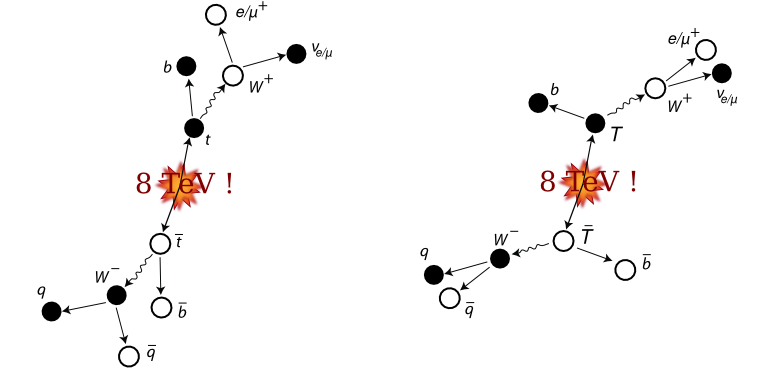
\includegraphics[width=0.85\textwidth]{wbx_analysis_14ifb/figures/kin}}
	\caption{Pictorial representation of the typical kinematic configuration
        for top pairs decays (left), where the boosted objects are the top
        quarks themselves, and vector-like top pairs decays (right), where the
        boosted objects are the $W$ bosons.\label{fig:boostedkin}}
\end{center}\end{figure}

In order to exploit this dynamic the angular separation of the final state
objects is considered. Since the $W$ boson decay
in the lepton channel cannot be completely resolved because of
the presence (or better, absence) of a neutrino, the analysis
focuses on the reconstruction of the $W$ boson that decays in the hadronic
channel, called \whad\ in the following.
The two jets from the decay of the \whad\ are expected to be
light flavored jets. At the preselection level at least
one \btag ged jet is required. Since two \btag ged jets are expected in
the final state and in order to avoid the loss in acceptance that would follow a strict
cut like requiring at least two \btag ged jets, the two jets with the 
highest weight computed from the \btag ging algorithm are considered ``\bjet s''.
Amongst the light jets two cases are considered: either the two light flavoured
quarks were produced so close-by that after hadronization the jet reconstruction
algorithm identifies a single jet, or two jets are found close one to the other.
To account for the first category of events, jets with $\pt>250\gev$ and a mass
between 60~\gev\ and 120~\gev, an interval chosen to cover both the world-average 
$W$ and $Z$ boson masses values of $m_W = 80.4$~\gev\ and $m_Z = 91.2$~\gev\ and
hence increasing the acceptance for $T\to Zt$ events, are 
classified as \wi\ candidates. If no \wi\ candidates are found, jets are paired
in di-jet systems if their angular separation $\dr(j,j)$ is lower than 0.8 and, if
$p_T(jj)>200\gev$ and 
their invariant mass $m_{jj}$ lies in the same window as for the \wi\ candidates, they 
are taken as a \wii\ candidate.


\section{Control regions}\label{sec:wbxCR}

\section{Event selection}\label{sec:wbxEVT}

\section{Final discriminant: heavy quark reconstructed mass}\label{sec:wbxDISCR}

%\section{}\label{sec:}

\section{Systematics}\label{sec:wbxSYS}

%\subsection{Technical Details}
The general aspects of the systematic uncertainties considered
in the \wbx\ and \htx\ analyses were illustrated
in Section~\ref{sec:systematics}, here the traits specific to the
\wbx\ analysis will be described.

\subsection{Merging of non-$t\bar{t}$ Backgrounds}

The very stringent cuts defined to select signal and reject
background work so well that very low statistics is left for
``non-$t\bar{t}$'' backgrounds ($W+$jets, $Z+$jets, dibosons, single top, 
$t\bar{t}V$)\footnote{The prediction for QCD multi-jet background contribution
is negative and consistent with zero and is then set to zero.}.
This can lead to problems with the treatment of some systematic uncertainties as
e.g. an empty bin in the nominal case might have non-zero content in the
systematically varied sample. For this reason, considering that no resonances
are expected for these backgrounds, these \nontt\ samples are merged into
a single component. Systematic uncertainties like cross-section normalization,
which are specific for each background, are applied to the single component
and the nominal version of the other samples are added to obtain
a varied histogram.
For the \nontt\ background all systematic uncertainties are
treated as normalization-only.

%Contrary to what was described in Table~\ref{tab:sys}, all systematics are considered as normalization only for this small-background component. For the {\sc Tight} selection, we take the values derived from the {\sc Loose} selection, as we do not expect significant difference between the two cases.

\subsubsection{Statistical uncertainty of the MC samples???}
The statistical uncertainty of the MC samples is taken into account when computing our likelihoods.
The {\sc mclimit} flag used is 2, meaning we consider the uncertainties as given by the uncertainties of the templates. 
This allows us to correctly estimate the statistical uncertainty when many templates are merged together with different weights, such as in
the case of the merged non-$t\bar{t}$ background.

\subsubsection{Profiling of Systematic Uncertainties}

No systematic uncertainty is profiled in the analysis, except for the overall 
$t\bar{t}$ yield in the {\sl loose} channel, exploiting the well defined 
sideband region at low $M_{reco}$ that is dominated by the \ttbar\ background
contribution. No profiled parameters are used in the {\sl tight} analysis.

\begin{table}[htb]
\centering
\caption{List of all systematic uncertainties (in \%) considered in the analysis, indicating which ones are treated
as normalisation and/or shape uncertainties, with their impact on normalisation in the case of the 
{\sl tight} selection, for signal and backgrounds. The signal given here is a chiral fourth-generation $T$ quark with mass $m_{T}=600\gev$.}
\begin{tabular}{l*{3}{c}}
\hline\hline
 & $\T\bar{\T}$ ($600\gev$) \rule{0pt}{2.6ex} \rule[-1.2ex]{0pt}{0pt} & $t\bar{t}$ & Non-$t\bar{t}$\\
\hline
\multicolumn{4}{c}{Uncertainties [\%] affecting only the normalisation of the $m_{\rm reco}$ distribution:}\\
Luminosity & +3.6/-3.6 & +3.6/-3.6 & +3.6/-3.6\\
Lepton trigger, reconstruction and ID efficiency & +2.0/-2.0 & +2.0/-2.0 & +2.0/-2.0\\
$t\bar{t}$ cross section & -- & +10/-11 & --\\
\hline
\multicolumn{4}{c}{Uncertainties [\%] affecting both normalisation and shape of the $m_{\rm reco}$ distribution:}\\
Jet energy scale & +6.6/-8.4 & +15/-15 & +33/-22\\  
Jet energy resolution & +8.4/-8.4 & +3.6/-3.6 & +9.3/-9.3\\ 
Jet identification efficiency & +2.3/-2.7 & +2.3/-2.5 & +1.9/-2.6\\  
$b$-quark tagging efficiency & +6.7/-7.3 & +6.7/-8.9 & +1.8/-2.2\\  
$c$-quark tagging efficiency & +1.6/-1.6 & +4.1/-4.1 & +5.6/-5.6\\  
Light-jet tagging efficiency & +0.3/-0.3 & +0.7/-0.7 & +2.7/-2.7\\  
$t\bar{t}$ modelling: NLO MC generator & -- & +48/-48 & --\\  
$t\bar{t}$ modelling: parton shower and fragmentation & -- & +25/-25 & --\\  
$t\bar{t}$ modelling: initial and final state QCD radiation & -- & +8.8/-8.8 & --\\   
$W$+jets normalisation & -- & -- & +8.9/-7.8\\  
$W$+heavy-flavor fractions & -- & -- & +18/-19\\  
$W$+jets modelling: scale variation & -- & -- & +11/-11\\  
$Z$+jets cross section & -- & -- & +1.1/-1.1\\ 
Single top cross section & -- & -- & +1.9/-1.5\\  
Diboson cross section & -- & -- & $<0.1\%$\\  
$t\bar{t}V$ cross section & -- & -- & +1.5/-1.5\\  
\hline
Total & +14/-15 & +59/-59 & +42/-35\\
\hline\hline
\end{tabular}
%\caption{List of all systematic uncertainties (in \%) considered in the analysis, indicating which ones are treated
%as normalisation and/or shape uncertainties, with their impact on normalisation in the case of the 
%{\sl tight} selection, for signal and backgrounds. The signal corresponds to a chiral fourth-generation $\T$ quark with mass $m_{\T}=600\gev$.}
\label{tab:SystSummary}
\end{table}




%%%%%%%%%JES

Even with a single JES uncertainty, large unphysical bin-to-bin fluctuations are observed
in the $m_{\rm reco}$ distribution for $t\bar{t}$ and ``non-$t\bar{t}$" backgrounds in the {\sl tight} analysis,
when comparing the varied JES templates with the nominal one. To avoid injecting
noise in the statistical analysis, the same shape systematic as for the {\sl loose} analysis,
which is smoother owing to the higher-statistics MC templates, is applied to the {\sl tight} 
analysis in case of the $t\bar{t}$ backrground. In the case of the ``non-$t\bar{t}$" background,
which has a rather flat  $m_{\rm reco}$ distribution, the JES systematic is taken to be
flat, affecting only the overall acceptance but not the shape.
%Appendix~\ref{app:JEScomp} documents a study on the impact of each of the JES nuisance parameters on the normalisation and shape of the 
%reconstructed Higgs boson mass and $H_{Thad}$ distributions for $t\bar{t}H$ signal and $t\bar{t}$+jets background background in different
%jet multiplicity bins used in the analysis.
%Such study has resulted in a simplified prescription for the JES uncertainty breakdown for this analysis than involves a total
%of 9 nuisance parameters. 


%%%JER
In the case of the $t\bar{t}$ and ``non-$t\bar{t}$'' background the same treatment as for
JES (see Section~\ref{sec:syst_jes}) is applied in order to reduce the impact from
large statistical fluctuations in the estimated systematic.


\subsubsection{Jet Mass Scale and Resolution}
The jet mass is used  to identify the most energetic hadronically-decaying $W$ bosons that have been reconstructed as  single jets
($W_{\rm had}^{\rm type\;I}$ candidates). The uncertainties affecting the jet mass had been studied in the previous analysis at $\sqrt{s}=7\tev$ 
(see Section  8.2.7 in Ref.~\cite{atlas_WbWb_5fb_ljets_backup}. At the time, the existing jet mass scale/resolution uncertainties had been derived for larger anti-$k_t$ jets 
($R=1.0$) and in release 16~\cite{jet_mass_2011} and were believed to be conservative when applied to smaller $R=0.4$ jets using the 
refined calibration from release 17.  The jet mass scale uncertainties used in Ref.~\cite{atlas_WbWb_5fb_ljets_backup} were
4.5\% for jets with $\pt<400\gev$ and 6\% for $\pt>400\gev$ (from Table 18 in Ref.~\cite{jet_mass_2011}). The jet mass resolution
uncertainty used was 20\%, independent of jet $\pt$ (from Table 18 in Ref.~\cite{jet_mass_2011}). 
The propagation of these uncertainties in the previous analysis led to a degradation in the expected sensitivity of only a few $\gev$
(compare yellow and light blue curves in Fig. 25(b) of Ref.~\cite{atlas_WbWb_5fb_ljets_backup}). Given the small impact on the
sensitivity of an almost identical analysis at $\sqrt{s}=7\tev$ of what was judged to be a conservative uncertainty at the time, and since
no recommendation for  $R=0.4$ jets currently exists,  this uncertainty is currently being neglected.

\subsection{\Wboson/\Zboson+jets Normalisation}
\label{sec:syst_vjetsnormWBX}
The $W$/$Z$+jets cross sections from {\sc Alpgen} are affected by large uncertainties because they 
are a leading-order calculation. 
As discussed in Section~\ref{sec:wjets_bkg}, the overall $W$+jets normalisation is obtained via data-driven methods 
separately for events with exactly 4 jets and $\geq 5$ jets in order to ensure the best possible central value for the 
predicted $W$+jets yield. 
Additional uncertainties are considered on the fractions of $Wb\bar{b}$, $Wc\bar{c}$ and $Wc$,
as well as the their extrapolation from 2-jet events, where they are measured in data,  to higher jet multiplicity. 
The sum in quadrature of the above contributions result in a total uncertainty of $\sim$30\% on
the estimated $W$+jets normalisation for events satisfying the {\sl tight} selection.


\subsubsection{$t\bar{t}$ Modelling}
\label{sec:systematic_ttbarmodel}
A number of systematic uncertainties affecting the modelling of $t\bar{t}$ are considered
in this analysis: 
(1) the choice of NLO event generator,
(2) the modeling of initial and final state QCD radiation, and
(3) the choice of parton-shower and fragmentation models.

\paragraph{NLO Event Generator:}
The effect of uncertainties on the parton-level modeling of $t\bar{t}$ is obtained by comparing the distributions from two 
NLO MCs, {\sc MC@NLO} and {\sc PowHeg}, both interfaced to {\sc Herwig}.  This choice is based on detailed comparisons
between data and MC in a number of control regions, often defined starting from the {\sl loose} selection but with one of
the cuts inverted to reject a possible signal contribution. In these studies three different $t\bar{t}$ generators, {\sc MC@NLO}, {\sc PowHeg} and
{\sc Alpgen} were compared. In general, it was found that data was bracketed by {\sc MC@NLO} and {\sc PowHeg} predictions,
with {\sc MC@NLO} providing the best description overall, which motivated its choice as the main $t\bar{t}$ generator for this analysis. 
In contrast, {\sc Alpgen} was found to be the most inconsistent model with data, predicting yields above {\sc PowHeg}, which motivated its rejection
as a valid alternate $t\bar{t}$  model in the kinematic region explored by this analysis.

Differences between {\sc MC@NLO} and {\sc PowHeg} arise from 
the details on how the NLO calculation is interfaced with the parton shower, resulting in {\sc PowHeg} predicting higher
jet multiplicities than {\sc MC@NLO}. These two samples have been processed through a fast simulation.
The relative uncertainty between {\sc PowHeg}+{\sc Herwig} and {\sc MC@NLO} fast-simulation samples is symmetrised and propagated to the 
{\sc MC@NLO} fully simulated sample. The resulting uncertainty on the $t\bar{t}$ yield after the {\sl tight} selection is 48\%, and constitutes the
main source of uncertainty on the $t\bar{t}$ background. The corresponding uncertainty after the {\sl loose} selection is 16\%. The significant
increase in the uncertainty for the {\sl tight} selection primarily results from the increased jet multiplicity in {\sc PowHeg} compared to {\sc MC@NLO}, 
which leads to a larger rate of misreconstruction of the $W_{\rm had}$ candidate, and renders the $\min(\Delta R(W_{\rm had}, b_{1,2}))>1.4$ cut less 
effective than in the case of  {\sc MC@NLO}.

\paragraph{Initial- and Final-State QCD Radiation:}
To assess the systematic uncertainty on the modeling of initial-state (ISR) and final-state radiation (FSR), dedicated
$t\bar{t}$ samples are generated with {\sc AcerMC}+{\sc Pythia} with modified {\sc Pythia} parameters 
\ifIsINT
(PARP(67), PARP(64) and PARP(72)) 
\fi
in order to increase or reduce the amount of parton shower. 
\ifIsINT
These alternate samples are referred to as ``morePS" and ``lessPS", respectively.
\fi
The range of variation for these parameters is chosen to be consistent with existing measurements such as the gap fraction in dileptonic 
$t\bar{t}$ events~\cite{ttjet}  and jet shapes in QCD multijet events.
\ifIsINT
For more details see Ref.~\cite{morelessPS}.  
\fi
These samples have been processed through a fast simulation. Half the difference between these alternate samples is symmetrised 
and propagated to the {\sc MC@NLO} fully-simulated sample, resulting in an uncertainty on the $t\bar{t}$ yield after the {\sl tight} selection of 8.8\%.

\paragraph{Parton-Shower and Fragmentation Models:}
Uncertainties on the simulation of the parton shower and fragmentation are studied comparing
two different hadronisation models applied to the same parton level generator: {\sc PowHeg}+{\sc Herwig} vs {\sc PowHeg}+{\sc Pythia}. 
These two samples have been processed through a fast simulation.
The relative uncertainty between {\sc PowHeg}+{\sc Herwig} and {\sc PowHeg}+{\sc Pythia} fast-simulation samples is symmetrised and propagated to the 
{\sc MC@NLO} fully simulated sample, resulting in an uncertainty on the $t\bar{t}$ yield after the {\sl tight} selection of 25\%. 

\ifIsINT
\vspace{1cm}
The limited available MC statistics in the {\sl tight} selection result in large bin-to-bin fluctuations and unphysical shape systematics.
In order to try to get smoother uncertainties the following procedure is followed:
\begin{enumerate}
\item estimate acceptance change by comparing the alternative MC samples;
\item compute ratio of unit-normalized templates from the alternative MC samples (they are statistically-independent) to derive shape
         distortion, and fit it with a low-order polynomial. In the case of the NLO generator systematic, the ratio is consistent with flat so this
         uncertainty in taken to affect only normalization (the first bin in the template contains very little statistics in data and MC, so it's not
         numerically relevant to account for the larger effect); in the case of the ISR/FSR and fragmentation systematics, a first-order polynomial
         is used for the paramerization. See fits in Fig.~\ref{fig:ttbarmodel_ratios}.
\item multiply the nominal template by each of the parameterizations obtained in 2) and normalize its yield with the relative acceptance changes found in 1).
          The resulting shape systematics can be found in Appendix~\ref{sec:TOPMODEL}.
\end{enumerate}

%%%%%%%%%%%%%%
\begin{figure}[htbp]
\begin{center}
\begin{tabular}{ccc}
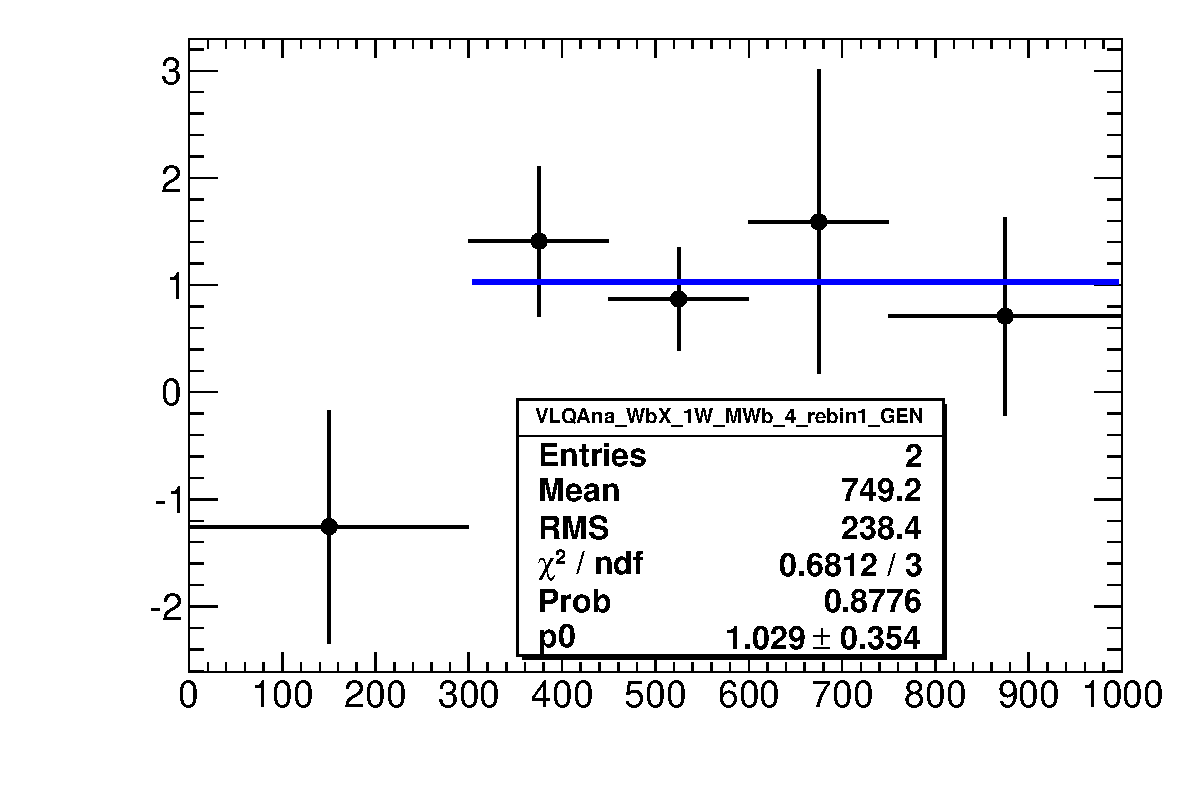
\includegraphics[width=0.33\textwidth]{figures/ttbarModRatio/GEN_RATIO.eps} &
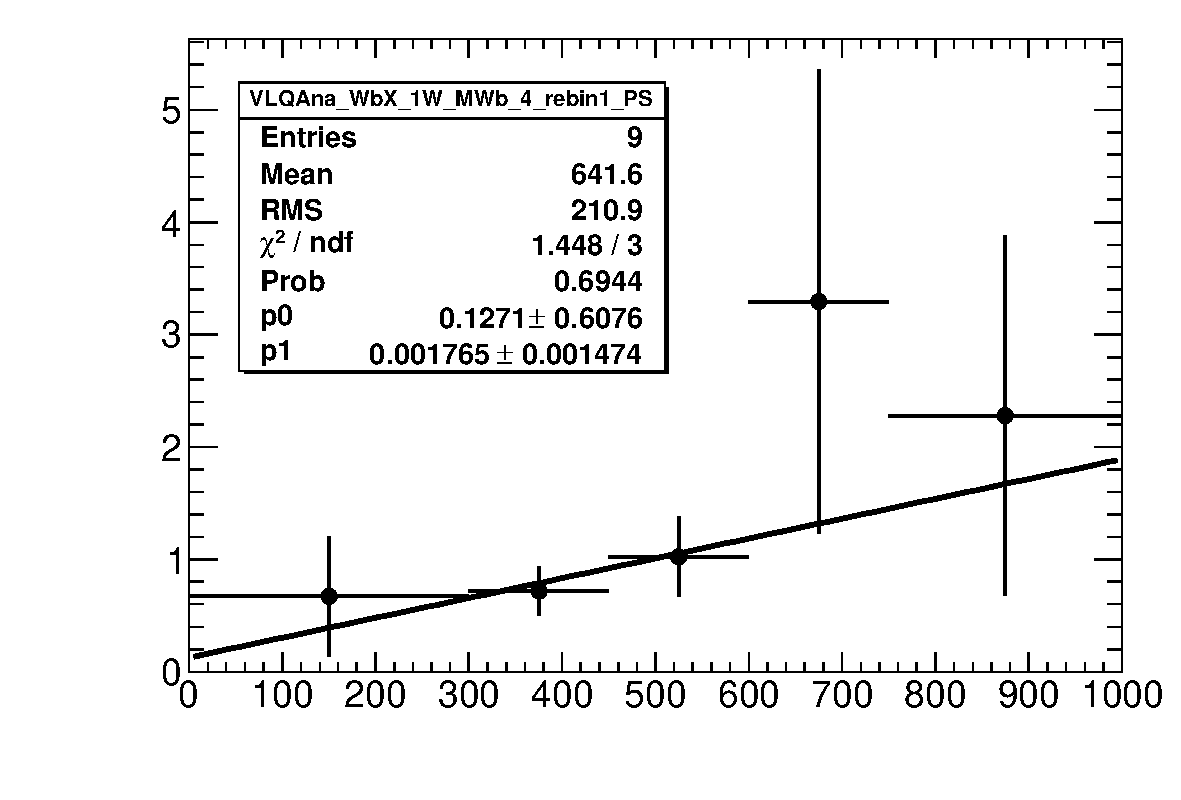
\includegraphics[width=0.33\textwidth]{figures/ttbarModRatio/PS_RATIO.eps} &
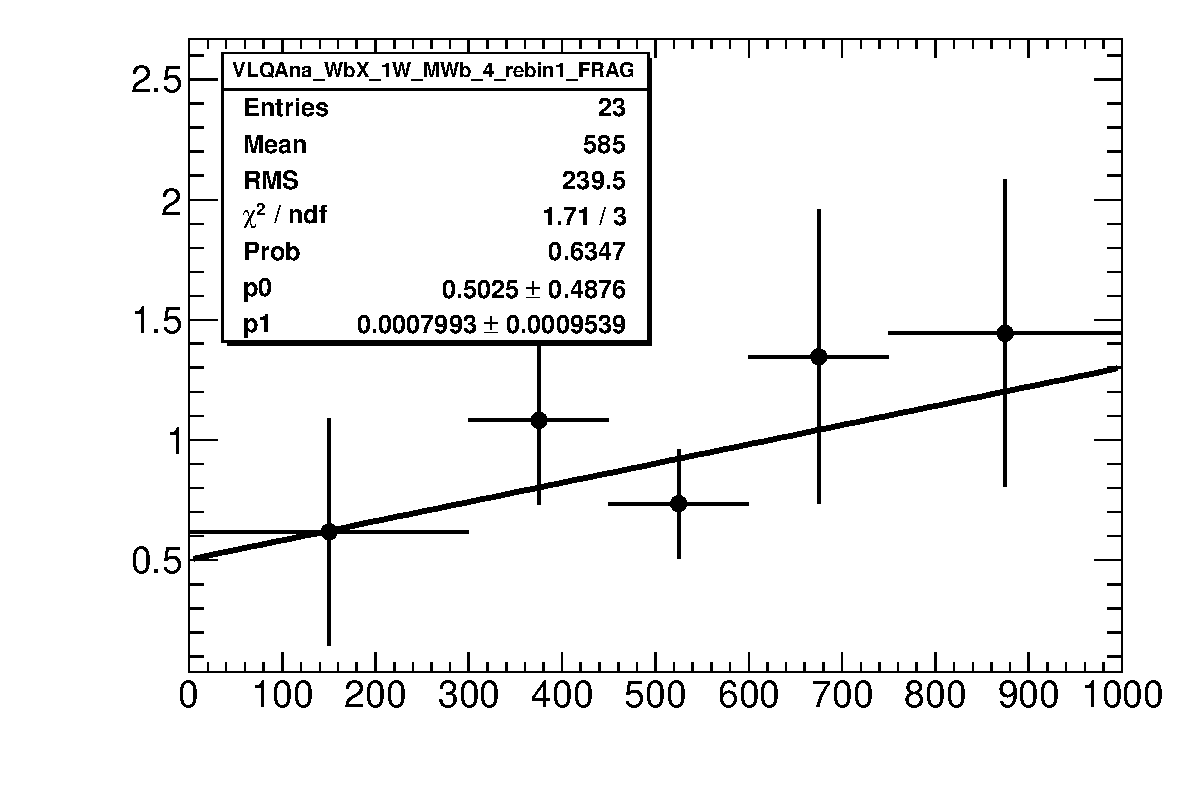
\includegraphics[width=0.33\textwidth]{figures/ttbarModRatio/FRAG_RATIO.eps} \\
(a) & (b) & (c) \\
\end{tabular}\caption{\small {Ratio of unit-normalized final discriminant between alternative models:
(a) {\sc mc@nlo} /{\sc PowHeg+Herwig}  to derive the NLO event generator systematic,
(b) {\sc AcerMC+lessPS} /{\sc AcerMC+morePS}  to derive the NLO event generator systematic, and
(c) {\sc PowHeg+Herwig} /{\sc PowHeg+Pythia}  to derive the parton shower+fragmentation systematic.
All samples used are AFII.
Also shown are fits to low-order polynomials in order to derive smooth shape systematics.}}
\label{fig:ttbarmodel_ratios}
\end{center}
\end{figure}
%%%%%%%%%%%%%%
\fi

\subsubsection{$V$+jets Modelling}
\ifIsINT 
The effect of uncertainties in the modeling of $V$+jets kinematics by {\sc Alpgen}  is assessed by varying a number of {\sc Alpgen} 
generator parameters. 
The Top Group recommended variations are changing the factorization scale from the nominal
choice $Q^2 =m_{\rm W}^2+\sum m_{\rm T}^2$ (default) to $Q^2 =m_{\rm W}^2+p_{\rm T,W}^2$  (iqopt3) and reducing the
minimum parton $\pt$ from $15\gev$ (default) to $10\gev$ (ptjmin10). 
\else
The effect of uncertainties in the modeling of $V$+jets kinematics by {\sc Alpgen}  is assessed by changing the factorization scale from the nominal
choice, $Q^2 =m_{\rm W}^2+\sum m_{\rm T}^2$, to $Q^2 =m_{\rm W}^2+p_{\rm T,W}^2$. This uncertainty is then symmetrised.
\fi
\ifIsINT 
The variations are implemented via a per-event weight computed as a function of leading jet $\pt$. For more information see Ref.~\cite{WjetsReweighting}.
{\bf Caveat: currently only the iqopt3 uncertainty is being considered. The ptjmin10 uncertainty will be included in the next iteration.}
\fi
